\documentclass[10pt,conference]{IEEEtran}

\makeatletter
\def\ps@headings{%
\def\@oddhead{\mbox{}\scriptsize\rightmark \hfil \thepage}%
\def\@evenhead{\scriptsize\thepage \hfil \leftmark\mbox{}}%
\def\@oddfoot{}%
\def\@evenfoot{}}
\makeatother
\pagestyle{headings}

% Load basic packages

\usepackage{amsmath}
\usepackage{balance}  % to better equalize the last page
\usepackage{graphicx}
\usepackage{subfigure}
\usepackage{graphics} % for EPS, load graphicx instead
\usepackage{times}    % comment if you want LaTeX's default font
\usepackage[hyphens]{url}      % llt: nicely formatted URLs
\usepackage{array}
\usepackage{enumerate}
\usepackage{algorithm2e}
\usepackage{color}
\usepackage{comment}
%\usepackage[bookmarks=false]{hyperref}


\newcommand{\todo}[1]{\textcolor{red}{TODO: #1}\\}

% llt: Define a global style for URLs, rather that the default one
%  \makeatletter
%  \def\url@leostyle{%
%   \@ifundefined{selectfont}{\def\UrlFont{\sf}}{\def\UrlFont{\small\bf\ttfamily}}}
%  \makeatother
%  \urlstyle{leo}


% To make various LaTeX processors do the right thing with page size.
\def\pprw{8.5in}
\def\pprh{11in}
\special{papersize=\pprw,\pprh}
\setlength{\paperwidth}{\pprw}
\setlength{\paperheight}{\pprh}
\setlength{\pdfpagewidth}{\pprw}
\setlength{\pdfpageheight}{\pprh}

% Make sure hyperref comes last of your loaded packages,
% to give it a fighting chance of not being over-written,
% since its job is to redefine many LaTeX commands.

% \usepackage[pdftex]{hyperref}
% \hypersetup{
% pdftitle={SIGCHI Conference Proceedings Format},
% pdfauthor={LaTeX},
%   pdfkeywords={SIGCHI, proceedings, archival format},
%   bookmarksnumbered,
%   pdfstartview={FitH},
%   colorlinks,
%   citecolor=black,
%   filecolor=black,
%   linkcolor=black,
%   urlcolor=black,
%   breaklinks=true,
% }

% create a shortcut to typeset table headings
\newcommand\litem[1]{\item{\bfseries#1\space:\space}}
\newcommand\tabhead[1]{\small\textbf{#1}}
\newcommand{\squeezeup}{\vspace{-3mm}}
\renewcommand{\labelitemi}{$\bullet$}
\renewcommand{\labelitemii}{$\cdot$}
\renewcommand{\labelitemiii}{$\diamond$}
\renewcommand{\labelitemiv}{$\ast$}
%\newcommand{\todo}[1]{\textcolor{red}{TODO: #1}}

\begin{document}
\title{SSD : Supervised Sarcasm Detection in Twitter using Social Cues}
%: Semi-Supervised Recognition of Sarcastic Sentences
%in Twitter and Amazon (CoNLL '10)}

\author{\IEEEauthorblockN{Swadhin Pradhan, Jian He}
\IEEEauthorblockA{CS, The University of Texas at Austin}}
% \IEEEauthorblockA{\IEEEauthorrefmark{2}CSE Department, Indian Institute of Technology Kharagpur, India}
% \IEEEauthorblockA{\IEEEauthorrefmark{3}CS Department, SUNY Korea}}


\date{20 April 2015}

\maketitle

%\renewcommand{\baselinestretch}{0.9}

\begin{abstract}
This project proposes a system for automatically detecting different facial expressions of a user using EEG and accelerometer data recorded in a headband like \textit{Muse}. We observe that different channels of EEG combined with accelerometer data exhibits specific patterns which can help to identify a specific set of facial expressions. These expression set may help to tag user generated content, e.g. comments on a forum or messages on a messenger (like Whatsapp), with actual emotions of users. Our key observation is that different sensors available on smartphones and different wearables like brainwave sensing headbands could be used to capture a wide spectrum of user reactions or emotions. Especially actual physiological signatures (EEG) captured by Muse \cite{muse}, which gives more detailed information about the user, can be critical in this regard. We can map these EEG, accelerometer and other sensor data captured to infer the current emotional states of user's mind. To achieve this, we have built a DTW based pattern matching algorithm which benefits from the low-rank structure of sensing data. Through experiments, we have shown that our system achieves reasonable accuracy for detecting expressions based on six expression vocabulary. 
\end{abstract}

\section{Introduction}
\todo{Abstract to be added}
\todo{Section reorientation also needed}

\noindent \textbf{Motivation :} Sarcasm is a form of speech act in which the speakers convey their message in an
implicit way. Sarcasm generally reverses the polarity of an utterance from positive or negative into its opposite. This inherently ambiguous nature of sarcasm sometimes makes it hard even for humans to decide whether an utterance is sarcastic or not. So, recognition of sarcasm can benefit many sentiment analysis NLP applications, such as review summarization,dialogue systems and review ranking systems \cite{Liu_survey}. Even recently FBI was also interested to find sarcastic tweets \cite{fbi_sarcasm} to improve their sentiment mining system.\\

\noindent \textbf{Dataset Collection and Description :} To collect a large-scale dataset from Twitter, we developed a distributed crawling platform to parallelize the crawling process. The open-source tool Tweepy was utilized to use APIs from Twitter application development framework. Twitter has limited each account to send $150$ requests within a $15$-min time window. To speed up the crawling process, we created $7$ twitter accounts to send requests in parallel. Sarcastic tweet dataset consists of the recent $10k$ tweets containing hashtags \emph{\#sarcasm}. We collected comprehensible information for each tweet, including the tweeter, tweet text, post time, the count of favorites, the count of retweets, etc. From these tweets, we further collect information for each tweeter. For each Twitter, we collected its follower count, followee count, user ID, status count, the list of followers, the list of followees, etc.
 
Please mention about Tweepy, Twitter rate limit, and creating 7 twitter accounts and corresponding apps for crawling. We have also used different 180 tweets annotated \cite{davidov10}, around 60k tweets \cite{tomas14} and also added different social information. Also describe a few more details.\\

\noindent \textbf{Discussion on Sarcastic Tweets: }Based on our observations, sarcastic tweets reveal both independent and dependent features. Generally, independent features characterize lexical or syntactic structures of tweets no matter who posted
them and what the content or topic of them is. While social network specific characteristics can reveal dependencies among tweets to some extent.

Lexical structures indicate similarities of using words or characters in raw text of tweets. The frequencies of punctuation, stopwords and slang represent one aspect of lexical structures. We explicitly utilize the occurrence of emoticons which are very closely related to sentiment representation of tweets. Moreover, hashtags and URLs are special lexicons in tweets, and they are possibly used to clarify the information conveyed in a sarcastic tweet. Some common phrases may be used to reverse the polarity of an utterance. Language models (such as Bigram, Trigram) are efficient ways to find out these phrases. Although twitter users think independently when updating their statues, certain level of similarities in lexical structures are expected to see due to their common intentions to represent sarcasms to their friends.

Compared with normal tweets, more complicated syntactic structures may appear in sarcastic tweets so that implicit meaning of them can be understood by others. The complexity of a syntactic tree can be represented by the number of nodes in the tree, the fraction of words appeared in the syntactic tree and the total words in tweet texts, etc. Syntactic complexity is an indicator of how easily the information of a tweet can be understood. Conventionally, sarcastic tweets convey messages implicitly, which possibly complicates syntactic structures.

Messages in social networks somewhat show some dependencies. On one hand, when people talk about a specific entity (such as a person, a movie, etc.), they tend to describe their opinions in similar ways. And we can always see common sentiments for some entities. For example, when someone wants to comment a movie, posting a sarcastic message can possibly invoke others' interests in following that message. Named entities represent the target or topic of a tweet. After recognizing named entities appeared in tweets, we are able to classify tweets into different types. For example, tweets about general events (such as weather) and tweets targeting at specific entities (like movies, actors, etc). Moreover, common sentiments towards specific entities can also possibly improve the accuracy of classification. The sentiment of the whole tweet is considered as the sentiment of named entities in that tweet. The number of named entities in a tweet also represents the intention that a user wants to convey complex messages. On the other hand, the social strength of a tweet can be defined as the number of favorites, retweets, the number of followers and followees the poster has. Generally, social strength can be considered as a factor which measures others' interests in a tweet. Posting sarcastic tweets is an efficient way to attract others' attention. Thus, tweets having higher social strength tend to be more likely sarcastic tweets. Exploiting dependencies can cluster tweets into several types having common properties. 


%Discuss in detail about different types of sarcastic tweets. My intuition says we may have seen mainly two types of sarcastic tweets : about general events (e.g. I like Mondays) and about named entity specific (e.g. I like Justin Beiber). Substantiate with clustering of tweets and trying different number of clusters with clustering functions.
\todo{Add some figures and Examples}\\

\noindent \textbf{Methodology :}
We need to describe our methodology and give some example of features.


\noindent \textbf{Features :}
\begin{itemize}
 \item Lexical Features
 \begin{itemize}
  \item Punctuation Frequencies
  \item Stopwords and Slang
  \item Emoticon Frequencies
  \item Capitalization
  \item Number of Hashtags and URLs
  \item Length of Sentence
 \end{itemize}

 \item Syntactic Features
  \begin{itemize}
  \item Relative frequencies of different POS tags (Tweebank and Tweeboparser)
  \item Cluster of POS Tags
  \item Fraction of words having syntactic function generated by syntactic trees of Tweeboparser
  \item Number of unique dependency root trees or inner nodes in trees of Tweeboparser
  \item Sentiment of the tweets using sentinet and Sentiment of hashtags
 \end{itemize}
 \item Social Features
  \begin{itemize}
  \item Named Entity and corresponding sentiment (comparing with the sentence sentiment)
  \item Strength of the tweet handlers (Favcount, Folower count, Folowee count etc.)
 \end{itemize}
\end{itemize}

\todo{We can also do Feature strength analysis using PCA}



%\input{eeg_primer}
%\section{Methodology and Experiment Setup}
\label{sec:methodology}
In this section, we will discuss in detail about umderlying working priniciples of SSD and different evaluation setups.
\subsection{Classifier Description}
We have initally attempted to train the system with simple unigram (bag of words), bigram, and tigram language model trained with $70\%$ of the tweets and testing with randomly selected $30\%$ of the tweets. For this binary classification task, we habe used SVM \cite{libsvm} with linear kernel and different ensemble techniques of boosting and bagging. Since we have a wide variety of features, we experimented with various ensemble learning techniques and found that LogitBoost performed best
empirically for boosting and bagging with SVM performed best for bagging technique. We used the Weka implementation of LogitBoost \cite{Friedman98} and EnsembleSVM for bagging \cite{ensembleSVM} to train a classifier using various combinations of features. We have used Decision Stumps as a base classifier in LogicBoost and ran boosting for 100 iterations. Furthermore, 
we have used SVM as a base classifier in bagging and ran bagging for 100 iterations. Training time of ensemble techniques were around $20$ hours in 8GB quadcore 3.2GHZ Ubuntu machine compared to around $1$ hour in SVM.

\subsection{Experiment Setup}

Fig. \ref{fig:infrastructure} shows the infrastructure of the whole system, which is divided into four parts: crawling module, parsing module, feature extracting module and sarcasm classifying module.

In the crawling module, we have developed a distributed crawling platform to collect a large-scale dataset from Twitter. The open-source tool Tweepy\cite{tweepy} was run on multiple machines in parallel, and all data will be centrally managed by the master node.

Raw tweets collected by the crawling module will be fed into the parsing module. The tool ark-twitter-nlp\cite{tweetnlp} was used to do tokenizing and POS tagging. After obtaining POS tagged tweets, TweeboParser\cite{kong2014dependency} will further run syntactic parsing which will generate syntactic dependency tree for each tweet. Named entity recognition was done by the tool in developed by Ritter et al\cite{Ritter11}\cite{Ritter12}. We applied sentiment analysis by utilizing the online machine learning framework Datumbox\cite{datumbox}. Due to the rate limit of this framework, we also created multiple parallel machine nodes to speed up sentiment analysis.

Parsed tweets are the input of the feature extracting module. We developed three feature extractors to extract corresponding features. After obtaining all tweet features, we are able to run the sarcasm classifying module, in which we used three classifiers, SVM with linear kernel, logitboosting with decision stump and bagging with SVM. 

\begin{figure}[htpb]
\centering
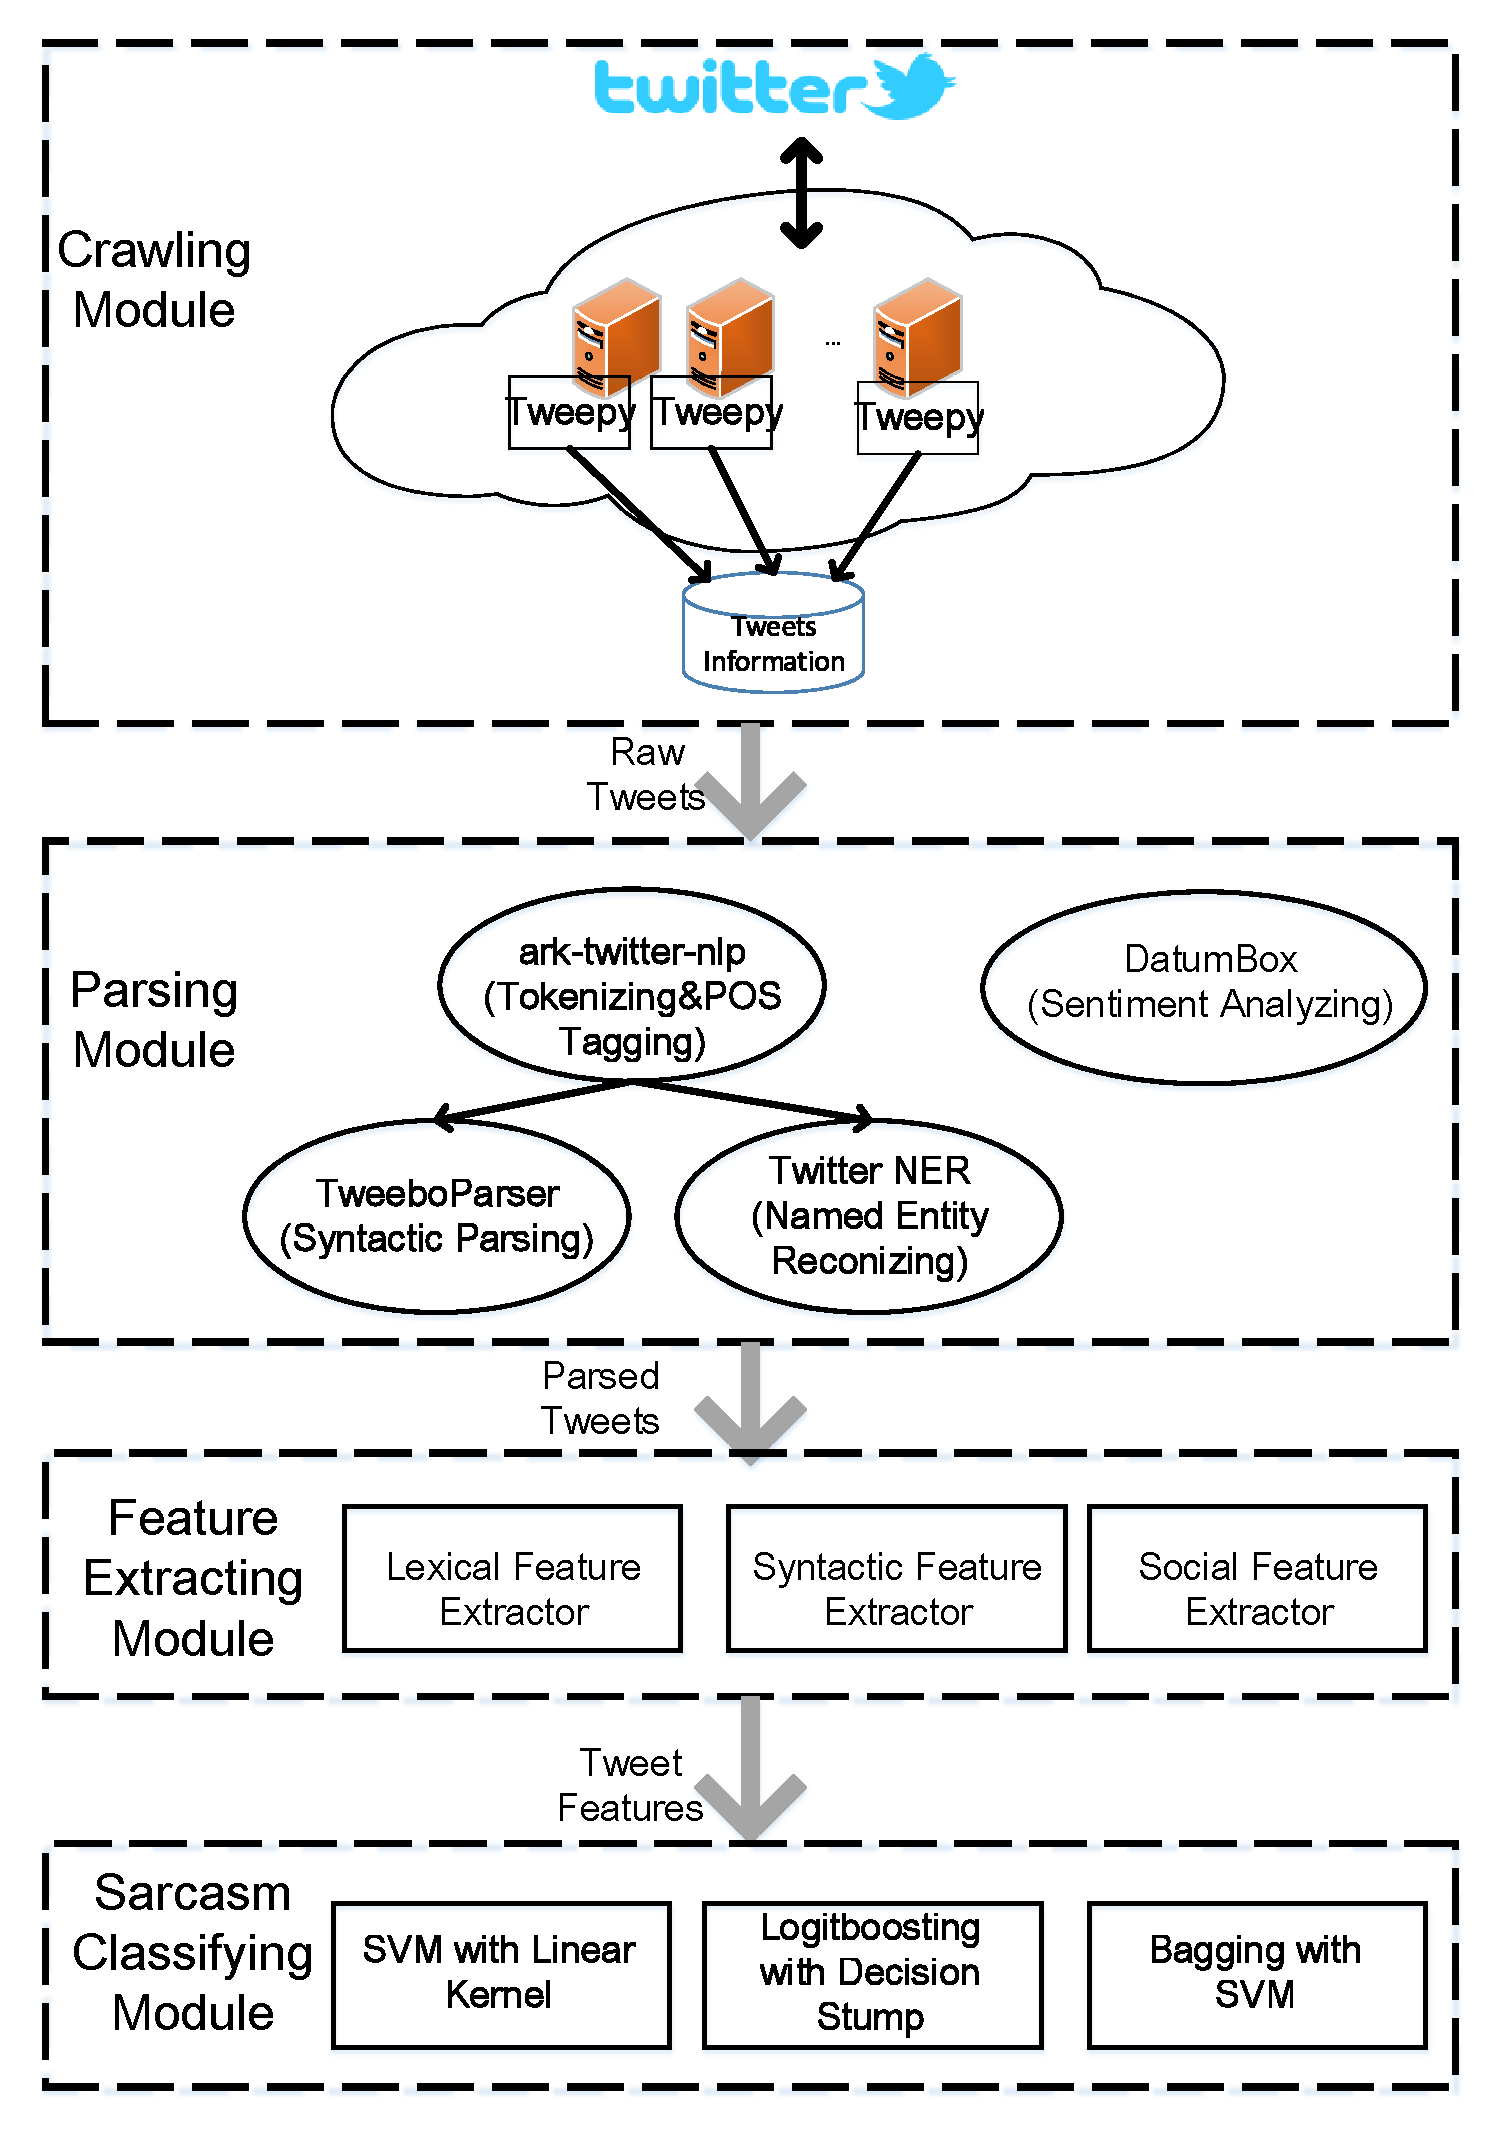
\includegraphics[scale=0.3]{infrastructure.eps}
\caption{The infrastructure of system setup.}
\label{fig:infrastructure}
\end{figure}

\section{Related Work}
\label{sec:related}
Sarcasm has been widely studied by psychologists, behavioral scientists and linguists for many years. Theories explaining the cognitive processes behind sarcasm usage such as the echoic reminder theory \cite{kreuz89}, allusional pretense theory \cite{kumon95}, and implicit display theory \cite{utsumi77} have been extensively researched. However, automatic detection of sarcasm is a relatively unexplored research topic and a challenging problem \cite{Pang2008}. While studies on automatic detection of sarcasm in speech \cite{tepper06} utilizes prosodic, spectral and contextual features, sarcasm detection in text has relied on identifying text patterns \cite{davidov10} and lexical features \cite{Kreuz07}.\\

Experiments with semi-supervised sarcasm identification on a Twitter dataset were conducted in \cite{davidov10}. They used 5-fold cross validation on their kNN-like classifier using mainly lexical features obtained an F-measure of 0.55 on the Twitter dataset. In \cite{davidov10}, authors use a semi-supervised sarcasm identification algorithm on a Twitter dataset and Amazon product reviews. In case of Twitter, authors mainly use $1500$ tweets containing \textit{\#sarcasm} hashtag and $180$ tweets tagged by $15$ Amazon Mechanical Turkers \cite{mturk} as golden test set or initial small labeled training set. The algorithm employs two modules: semi supervised pattern acquisition for identifying sarcastic patterns that serve as features for a classifier, and a classification stage that classifies each sentence to a sarcastic class. Reyes et al. \cite{reyes12} proposed features to capture properties of a figurative language such as ambiguity, polarity, unexpectedness and emotional scenarios. Their corpus consists of five categories (humor, irony, politics, technology and general), each containing 10,000 tweets. The best result in the classification of irony and general tweets was F-measure 0.65. Furthermore, Lukin and Walker \cite{Lukin_really13} explored the potential of a bootstrapping method for sarcasm classification in social dialogue to learn lexical N-gram cues associated with sarcasm (e.g., “oh really”, “I get it”, “no way”, etc.) as well as lexico-syntactic patterns. The work of Riloff et al. \cite{riloff13} identifies one type of sarcasm : contrast between a positive sentiment and negative situation. They used a bootstrapping algorithm to acquire lists of positive sentiment phrases and negative situation phrases from sarcastic tweets. Their evaluation on a human-annotated dataset of 3000 tweets (23\% sarcastic) was done using the SVM classifier with uni-grams and bigrams as features, achieving an F-measure of 0.48. \cite{gonzalez_acl} introduced a sarcasm detection technique using numerous lexical features (derived from LWIC \cite{pennebaker01} and Wordnet Affect \cite{valitutti04wordnet}) and pragmatic features such as emoticons and replies. Tomas et. al. \cite{tomas14} also tried to employ different combinations of machine learning approaches using language independent specific feature set on Czech and English Twitter dataset (780,000 tweets) and achieved F-measure around 0.94.
\section{Dataset Collection and Description}
\label{sec:dataset}
\subsection{Crawler Development}
To collect a large-scale dataset from Twitter, we developed a distributed crawling platform to parallelize the crawling process. The open-source tool Tweepy \cite{tweepy} was utilized to use APIs from Twitter application development framework. Twitter has limited each account to send $150$ requests within a $15$-min time window. To speed up the crawling process, we created $7$ twitter accounts to send requests in parallel. Sarcastic tweet dataset consists of the recent $10k$ tweets containing hashtags \emph{\#sarcasm}. We collected comprehensible information for each tweet, including the tweeter, tweet text, post time, the count of favorites, the count of retweets, etc. From these tweets, we further collect information for each tweeter. For each Twitter, we collected its follower count, followee count, user ID, status count, the list of followers, the list of followees, etc. Moreover, we have also collected non-sarcastic tweets of around $10k$ from different accounts.\\

Furthermore, we have contacted different authors \cite{davidov10,riloff13,tomas14} for similar works for twitter dataset, but they were unable to provide contents of tweets due to new Twitter terms of services \cite{twitter_tos}. Instead, authors \cite{davidov10,riloff13,tomas14} have provided us twitter ids corresponding with their labeling (These labels are done either by Amazon Turkers or by independent human evaluators). Then, we used our crawlers to collect tweets from those tweet ids with their socio-contextual information (on an average $10\%$ of the tweets were either deleted or inaccessible). Finally, we are able to collect 180 tweets annotated from \cite{davidov10}, around 50k tweets from \cite{tomas14} and around 5k tweets from \cite{riloff13}. Thus, we consolidated twitter dataset of size $75,213$ tweets consisting $38,112$ sarcastic tweets.

\subsection{Dataset Description}
The whole dataset is divided into three parts: tweets information, user profiles and user social relationships.

Table \ref{tab:tweet information} shows the format of a tweet information record. Note that, we only list the information we have used in our experiments. A tweet record in our dataset also includes other information, such as user device, geo-location, etc. 

A user profile record consists of the user name, followers count, followees count and status count. Table \ref{tab:user profile} illustrates the format for a user profile record. Details of the user social relationship dataset can be seen in Table \ref{tab:social relationship}.

\begin{table}[htpb]
\centering
\begin{tabular}{|c|c|c|c|}
\hline
Tweeter  & Text  & Favoriates Count & Retweets Count \\
\hline
\end{tabular}
\vspace{0.01 in}
\caption{Format for tweet information dataset.}
\label{tab:tweet information}
\end{table}

\begin{table}[htpb]
\centering
\begin{tabular}{|c|c|c|c|}
\hline
User Name & Followers Count & Followees Count & Status Count \\
\hline
\end{tabular}
\vspace{0.01 in}
\caption{Format for user profile dataset.}
\label{tab:user profile}
\end{table}

\begin{table}[htpb]
\centering
\begin{tabular}{|c|c|c|}
\hline
User Name & Follower1, Follower2, $\cdots$ & Followee1, Followee2, $\cdots$ \\
\hline
\end{tabular}
\vspace{0.01 in}
\caption{Format for user social relationship dataset.}
\label{tab:social relationship}
\end{table}
\section{Features}
\label{sec:features}
We will use three different groups of features to help improve sarcasm detection accuracy, including lexical features, syntactic features, and social features. Table \ref{tab:lexical features} shows the lexical features we used in our experiments. Lexical features mainly capture lexical patterns of tweets, such as common word usage, phrases, etc. Syntactic features illustrated in Table \ref{tab:syn features} represent syntactic structures of tweets, such as the simple SVO pattern, etc. We exploit social features listed in Table \ref{tab:social features} to characterize dependencies across tweets. For example, tweets with similar named entities tend to have same sentiments.

\begin{table}[htpb]
\centering
\begin{tabular}{|l|}
\hline
\tabincell{l}{Punctuation Frequencies\\
(The ratio between the number of punctuation \\
and the total number of tokens)} \\
\hline
Stopwords and Slang  \\
\hline
Emoticon Frequencies \\
\hline
Capitalization \\
\hline
Number of Hashtags and URLs \\
\hline
\tabincell{l}{Length of Sentence \\
(The number of tokens)}\\
\hline
Language Models(Unigram, Bigram and Trigram) \\              
\hline
\end{tabular}
\vspace{0.03 in}
\caption{Lexical Features}
\label{tab:lexical features}
\end{table}

\begin{table}
\centering
\begin{tabular}{|l|}
\hline
\tabincell{l}{Relative frequencies of different POS tags\\
parsed by the tool TweetNLP\cite{tweetnlp}\\
(The size of the tagset is $25$)}\\
\hline
\tabincell{l}{Fraction of words having syntactic function\\
(Syntactic dependency trees are generated by \\
TweeboParser\cite{kong2014dependency},some tokens do not \\
have syntactic function, such as ``RT'', ``@'', hashtags, etc.)} \\
\hline
\tabincell{l}{Number of inner nodes in dependency trees\\
(Phrases in a tweet can be characterized by subtrees,\\
thus the number of inner nodes is a reliable indicator\\
of the syntactic complexity of a tweet)}\\
\hline
\tabincell{l}{Sentiment of tweets\\
(The sentiment of a tweet can be positive,\\
negative or neutral. The online machine learning\\
framework Datumbox\cite{datumbox} is used to analyze sentiment.)}\\
\hline
\end{tabular}
\vspace{0.03 in}
\caption{Syntactic Features.}
\label{tab:syn features}
\end{table}

\begin{table}[htpb]
\centering
\begin{tabular}{|l|}
\hline
\tabincell{l}{Named Entities(The number of Named Entities,\\
the length of each named entity, the sentiment of each\\
named entity)}\\
\hline
\tabincell{l}{Social strength(The number of favorites,\\
the number of retweets, the follower count of the tweet\\
handler, the followee count of the tweet handler)}\\
\hline
\end{tabular}
\vspace{0.03 in}
\caption{Social Features}
\label{tab:social features}
\end{table}

\section{Methodology and Experiment Setup}
\label{sec:methodology}
In this section, we will discuss in detail about umderlying working priniciples of SSD and different evaluation setups.
\subsection{Classifier Description}
We have initally attempted to train the system with simple unigram (bag of words), bigram, and tigram language model trained with $70\%$ of the tweets and testing with randomly selected $30\%$ of the tweets. For this binary classification task, we habe used SVM \cite{libsvm} with linear kernel and different ensemble techniques of boosting and bagging. Since we have a wide variety of features, we experimented with various ensemble learning techniques and found that LogitBoost performed best
empirically for boosting and bagging with SVM performed best for bagging technique. We used the Weka implementation of LogitBoost \cite{Friedman98} and EnsembleSVM for bagging \cite{ensembleSVM} to train a classifier using various combinations of features. We have used Decision Stumps as a base classifier in LogicBoost and ran boosting for 100 iterations. Furthermore, 
we have used SVM as a base classifier in bagging and ran bagging for 100 iterations. Training time of ensemble techniques were around $20$ hours in 8GB quadcore 3.2GHZ Ubuntu machine compared to around $1$ hour in SVM.

\subsection{Experiment Setup}

Fig. \ref{fig:infrastructure} shows the infrastructure of the whole system, which is divided into four parts: crawling module, parsing module, feature extracting module and sarcasm classifying module.

In the crawling module, we have developed a distributed crawling platform to collect a large-scale dataset from Twitter. The open-source tool Tweepy\cite{tweepy} was run on multiple machines in parallel, and all data will be centrally managed by the master node.

Raw tweets collected by the crawling module will be fed into the parsing module. The tool ark-twitter-nlp\cite{tweetnlp} was used to do tokenizing and POS tagging. After obtaining POS tagged tweets, TweeboParser\cite{kong2014dependency} will further run syntactic parsing which will generate syntactic dependency tree for each tweet. Named entity recognition was done by the tool in developed by Ritter et al\cite{Ritter11}\cite{Ritter12}. We applied sentiment analysis by utilizing the online machine learning framework Datumbox\cite{datumbox}. Due to the rate limit of this framework, we also created multiple parallel machine nodes to speed up sentiment analysis.

Parsed tweets are the input of the feature extracting module. We developed three feature extractors to extract corresponding features. After obtaining all tweet features, we are able to run the sarcasm classifying module, in which we used three classifiers, SVM with linear kernel, logitboosting with decision stump and bagging with SVM. 

\begin{figure}[htpb]
\centering
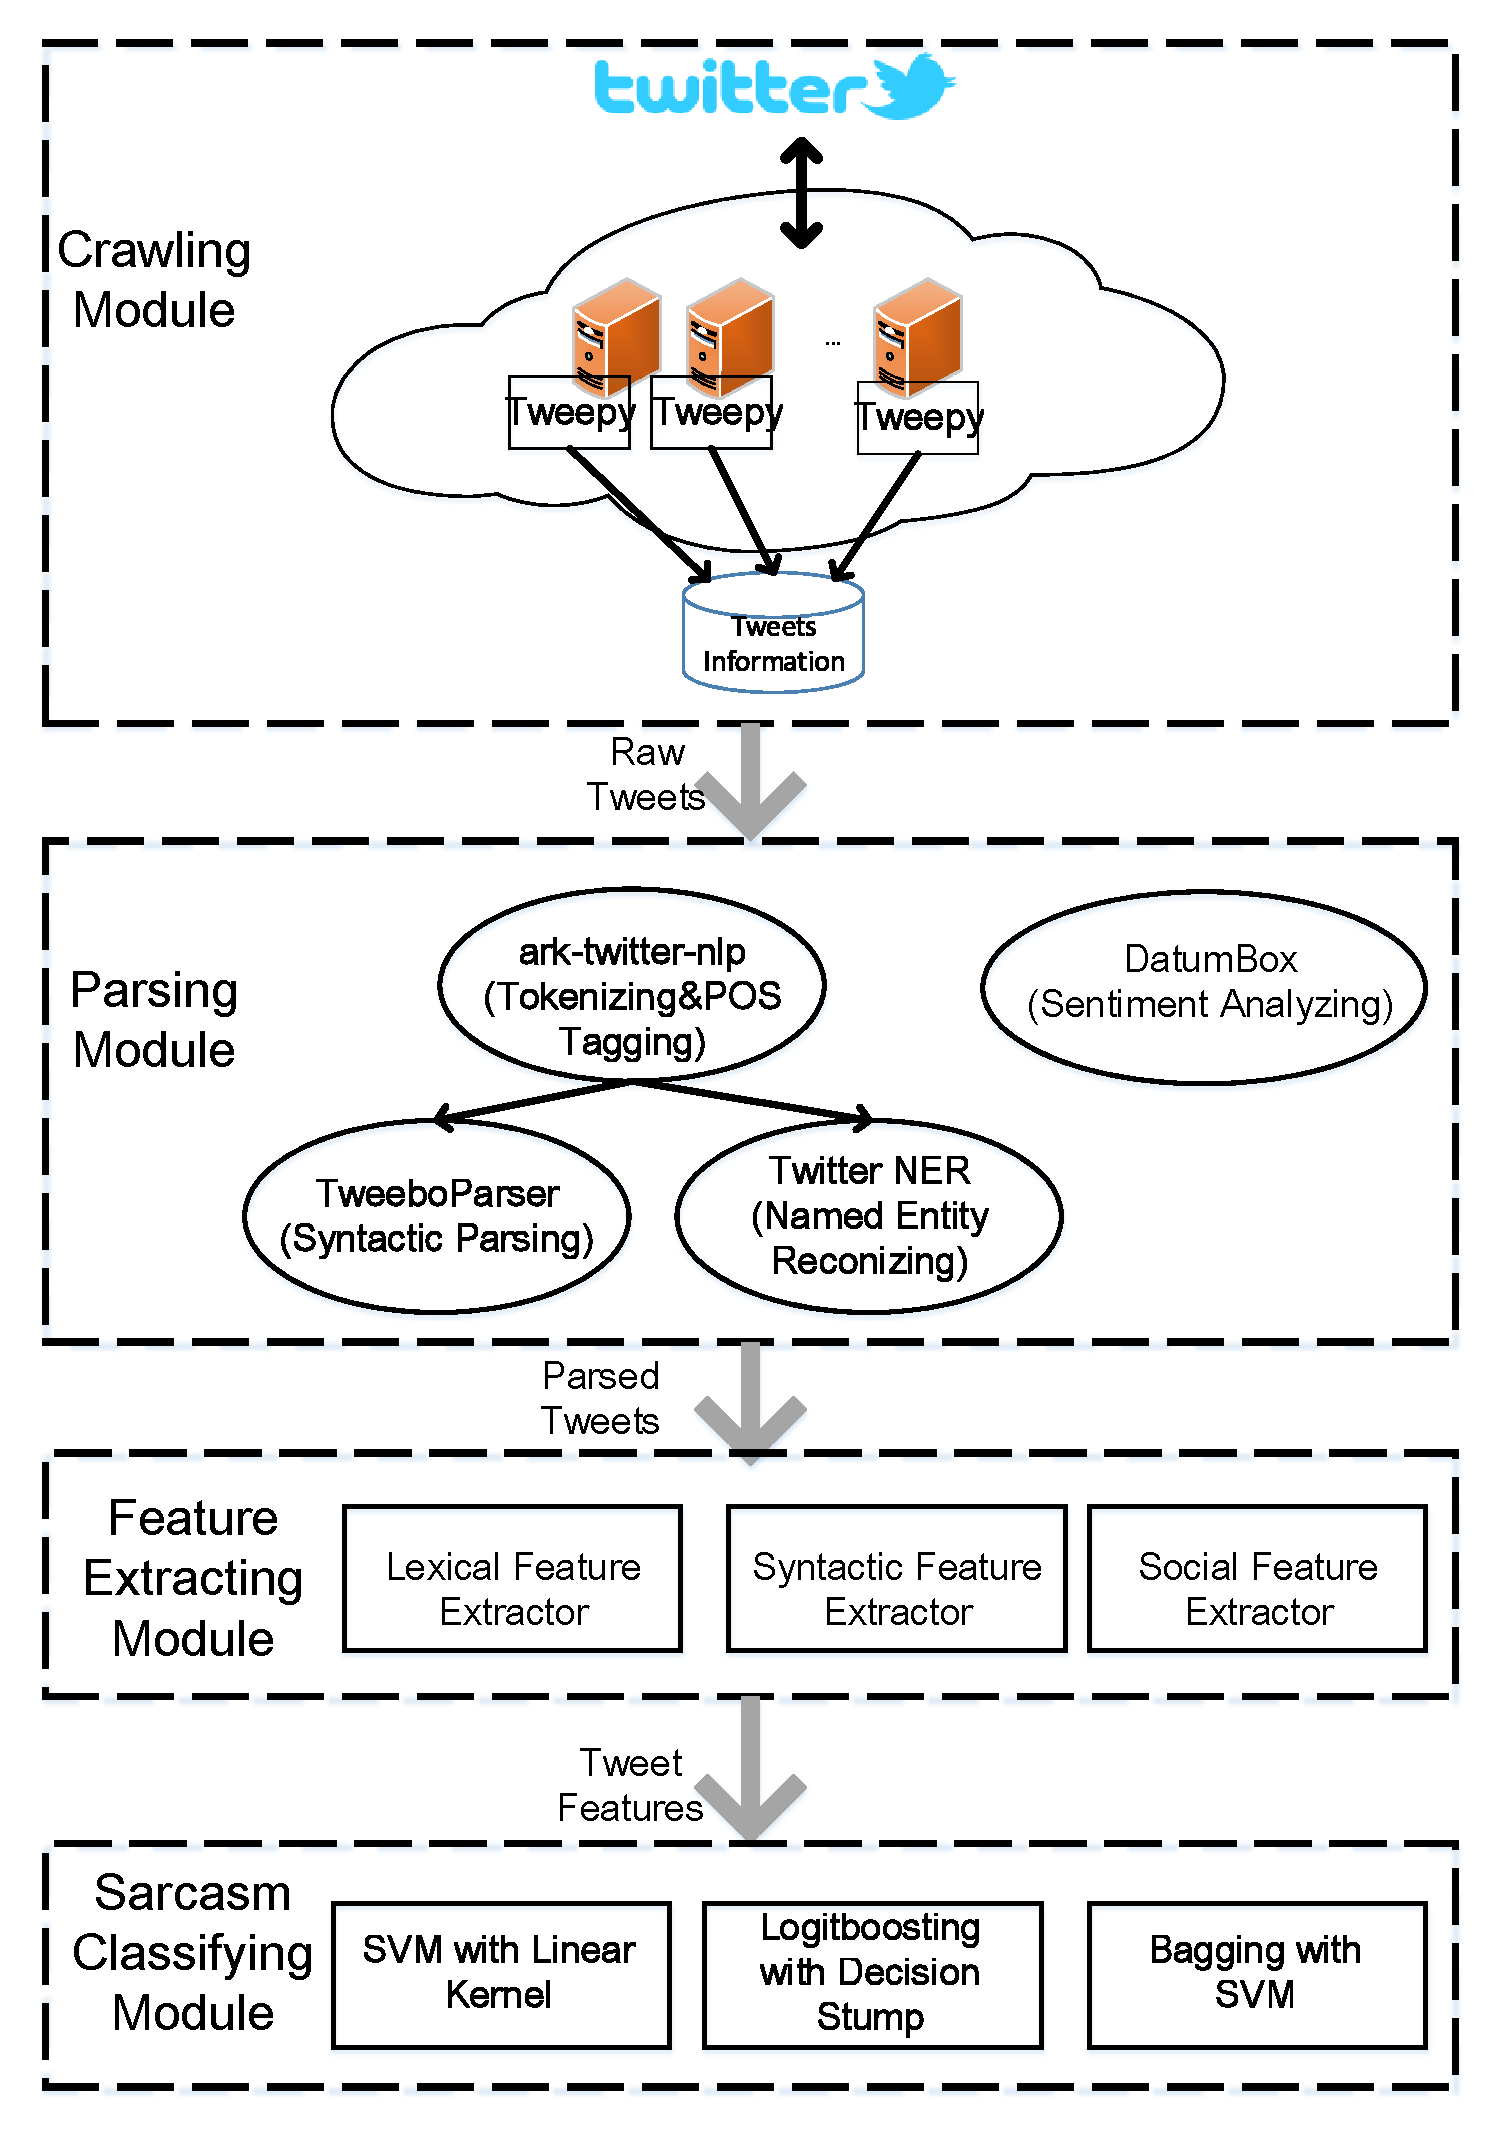
\includegraphics[scale=0.3]{infrastructure.eps}
\caption{The infrastructure of system setup.}
\label{fig:infrastructure}
\end{figure}

\section{Our Proposed Approach}
\label{sec:evaluation}
\noindent \textbf{Limitations of the Paper to be addressed :}
\begin{enumerate}
 \item Even the authors had 5.9 million tweets, they can only effectively use 1500 tweets as secondary training/test set and only 180 tweets as primary training/test set. Moreover, they achieve very poor precision of 0.545 in secondary dataset. So, in this project, we aim to crawl at least 10 thousand sarcastic tweets using Twitter's official search APIs via Tweepy \cite{tweepy} library. As there is rate limit to the apps per account in Twitter, we have already created multiple accounts to crawl in parallel to achieve the goal. If possible, we also hope to employ Amazon Mechanical Turk for data labelling and evaluation.
 \item In the paper, authors have not used any baseline for Twitter dataset as the semantic gap principle can not be easily adopted in case of Twitter. We aim to create a baseline for the Twitter dataset from this principle or some other recent work to compare our system's performance.
 \item Authors reduced the feature set for better pattern matching but they claim the better performance in Twitter dataset in second experiment is due to more number of features. So, the removal of hashtags, links etc. may reduce the context information (universal knowledge) in already restricted tweets of $140$ characters. We plan to gather the context information from the profile centric information of the users like follows, mentions, re-tweets, favorites, profile description, previous tweets etc. We believe that if we train any system with such context information then it will give better result in sarcasm detection as any kind of sarcasm assumes some sort of world knowledge.
 \item Interestingly, authors did not pursuit the idea of \textit{target} named entity in tweets as they did it in Amazon reviews. But, we believe that some classes of sarcastic tweets actually aimed at entities (e.g. may be person or institution or event or show) and if we can extract the sentiment regarding that we can get good indication of sarcasm. Moreover, some classes of sarcastic tweets may be general saying which is common across some classes of users (e.g. \textit{Yeah, I like Mondays more than my girlfriend}).
 \item Moreover, we can also use the lexical/morphological features like adding for example features based on latent semantics, topic models etc. to improve the accuracy, which the authors did not use. We may look at the effect of underlying social graph structure on the sarcastic nature of a particular tweet. Because, the social graph leaks the interest and expertise of the user and can hint at the tendencies of sarcasm to specific entities.\\
\end{enumerate}

\noindent \textbf{Main Idea :} In the discussed paper and all other relevant works, authors have attempted to classify tweets as an independent entity without incorporating the notion of world knowledge in some form. So, our intuition is that if we look into the user profile (In Twitter, some accounts are dedicated sarcastic fake accounts), his previous tweets, specific hashtags, specific mentions and the general sentiments of the named entities used in the tweet (e.g. \textit{Janet Jackson}, \textit{Twilight} the movie etc.), we can get more hints of the sarcastic nature of the tweets. Because, the restriction nature of tweets makes the outside contextual, temporal, and semantics meaning more important.\\

\noindent \textbf{Evaluation Plan :}
We have already collected the tweet sarcasm dataset used in \cite{davidov10} but it will not be readily used because the lack of any outside information. Moreover, we have also started to crawl \textit{Twitter} using search string \textit{\#sarcasm}, \textit{\#sarcastictweet}, and \textit{sarcasmimplied} via search API using tweepy\cite{tweepy} and collected around five thousand tweets. Thus, we plan to collect a reasonable amount of tweet with corresponding tweet centric information (like Geo IDs, Device IDs etc.), profile information, and one hop follower/followee information. Next, we plan to process all user, URL, hashtag, mention, emoticons of tweets according to the model of sarcasm detection mechanism. Tokenization of tweets requires proper handling of emoticons and other special character sequences
typical on Twitter which can be achieved using the ark-tweet-nlp tool \cite{gimpel11}. We also plan to extract named entity using Stanford Named Entity Recognition (NER) and also extract the sentiment about the entity collating all previous tweets about that entity. Next, we will try to use supervised machine learning algorithms like SVM, unsupervised algorithm like k-means clustering etc. with tuned and curated feature set. Finally, we will measure precision, recall, F-measure with different subset of features and investigate different trade-offs. 
\begin{table*}[htb]
%\renewcommand{\arraystretch}{1.9}
  \centering
  {\small
    %\vspace{-0.1in}
  \begin{tabular}{|@{~}l@{~~}|@{~~}l@{~}|@{~~}l@{~}|@{~~}l@{~}|@{~~}l@{~}|@{~~}l@{~}|@{~~}l@{~}|}
\hline
Dataset & Method Used & Precision & Recall & F1-Score & Area under Curve (AUC) & Testing Runtime \\\hline
Bag-of-Words & SVM & $88.9$ & $86.64$ & $24.03$ & $3.00$ & $7.05$ sec. \\\hline
Bigram & SVM & $99.87$ & $92.75$ & $33.01$ & $3.00$ & $83.6$ sec. \\\hline
Trigram & SVM & $99.88$ & $94.29$ & $48.77$ & $3.00$ & $87.43$ sec. \\\hline
Only Lexical Feature & SVM & $86.08$ & $78.27$ & $37.84$ & $15.32$ & $5$ min. $30$ sec. \\\hline
Only Syntactic Feature & SVM & $98.56$ & $79.41$ & $47.54$ & $15.32$ & $611$ min. $47$ sec.\\\hline
Only Social Feature & SVM & $99.13$ & $88.68$ & $78.97$ & $15.32$ & $591$ min. $23$ sec. \\\hline
All Features & SVM & $88.58$ & $83.18$ & $39.60$ & $11.40$ & $25$ min. $41$ sec. \\\hline
Bag-of-Words & Logicboost & $88.9$ & $86.64$ & $24.03$ & $3.00$ & $7.05$ sec. \\\hline
Bigram & Logicboost & $99.87$ & $92.75$ & $33.01$ & $3.00$ & $83.6$ sec. \\\hline
Trigram & Logicboost & $99.88$ & $94.29$ & $48.77$ & $3.00$ & $87.43$ sec. \\\hline
Only Lexical Feature & Logicboost & $86.08$ & $78.27$ & $37.84$ & $15.32$ & $5$ min. $30$ sec. \\\hline
Only Syntactic Feature & Logicboost & $98.56$ & $79.41$ & $47.54$ & $15.32$ & $611$ min. $47$ sec.\\\hline
Only Social Feature & Logicboost & $99.13$ & $88.68$ & $78.97$ & $15.32$ & $591$ min. $23$ sec. \\\hline
All Features & Logicboost & $88.58$ & $83.18$ & $39.60$ & $11.40$ & $25$ min. $41$ sec. \\\hline
Bag-of-Words & Bagging & $88.9$ & $86.64$ & $24.03$ & $3.00$ & $7.05$ sec. \\\hline
Bigram & Bagging & $99.87$ & $92.75$ & $33.01$ & $3.00$ & $83.6$ sec. \\\hline
Trigram & Bagging & $99.88$ & $94.29$ & $48.77$ & $3.00$ & $87.43$ sec. \\\hline
Only Lexical Feature & Bagging & $86.08$ & $78.27$ & $37.84$ & $15.32$ & $5$ min. $30$ sec. \\\hline
Only Syntactic Feature & Bagging & $98.56$ & $79.41$ & $47.54$ & $15.32$ & $611$ min. $47$ sec.\\\hline
Only Social Feature & Bagging & $99.13$ & $88.68$ & $78.97$ & $15.32$ & $591$ min. $23$ sec. \\\hline
All Features & Bagging & $88.58$ & $83.18$ & $39.60$ & $11.40$ & $25$ min. $41$ sec. \\\hline
%\vspace{-0.15in}
\end{tabular}
  }
 \vspace{0.05in}
  \caption{Summary of Results for running SVM, Boosting, and Bagging with different feature sets on datasets.}
%\vspace{-0.25in}
  \label{tab:data1}
\end{table*}

\section{Future Works}
\label{sec:future}
In this project, our goal was to capture the context of tweets in a holistic manner. To achieve this, one immediate future direction might be to get previous tweets of a user to get a better behavioral model which might help in prediction. We can also better model the persona or community of a twitter handle if we also can mine the interest from his follower list and previous retweets/mentions/favorites. Similarly, we can also get previous tweets belonging to particular topic or named entity mentioned in the tweet and get to know the general sentiment. If the general sentiment is negative, then any positive tweet, with high probability, might be sarcastic. Furthermore, in future, we will also attempt to get information about the topics or entities from outside sources such as search APIs. On the other hand, we can develop a hierarchical classifier for different types of sarcastic tweets which will initially predict the class of sarcastic tweet (e.g. general or entity specific) and then employ a class specific model to predict the sarcasm. We believe that this type of topical or socio-contextual model will help in predicting sarcastic tweets in a language independent way and can overcome the low F1-score reported in Czech dataset in \cite{tomas14}. Moreover, as \#sarcasm hashtag is a bit noisy, in future, we will try to employ amazon mechanical turkers for more confidence in judgment. We also should have investigated the importance of different features in terms of information gain.
%\input{emoapp}
%\input{path_forward}
%\section{Related Work}
\textbf{Image based Facial Expression Detection : }In the past years, the literature on automatic facial expression recognition has grown dramatically by applying advanced techniques of image and video processing. Most studies of automatic facial expression recognition focus on six primary facial expressions or a subset of them, namely happiness, sadness, anger, fear, surprise, and disgust. The expression and recognition of these primary facial expressions were found in Ekman’s extensive studies\cite{ekman} to be universal in different cultures. The studies of computer-assisted recognition of facial expressions started in 1990s. Mase\cite{mase} explored the technique of optical flow for facial expressions recognition. Lanitis et al.\cite{lanitis} applied a flexible shape and appearance model to recognize person identities, genders and facial expressions. Black and Yacoob\cite{black95} used local parameterized models of image motion to track non-rigid facial motion that was fed to a rule-based classifier of facial expressions. Rosenblum et al.\cite{rosenblum} used optical flow and a radial basis function network to
classify expressions. Otsuka and Ohya\cite{otsuka97} used optical flow and a hidden Markov model (HMM) for facial expression
recognition. Tian et al\cite{tian} explored action unit recognition by using multi-state facial component models and a neural-network-based classifier. Cohen et al.\cite{cohen03} introduced the structure of Bayesian network classifiers and a multi-level HMM classifier to automatically segment an arbitrary long sequence to the corresponding facial expressions. For extensive survey of facial expression analysis using images done in the recent years, readers are referred to the overview papers, including \cite{pantic00,pantic03} written by Pantic and Rothkrantz in 2000 and 2003.\\

\textbf{EEG based Expression and Emotion Detection : }Several works have attempted recognition of emotions from EEG signals. In \cite{channel2009}, participants are asked to remember an episode in their life that corresponds to positive/excited and one that corresponds to negative/excited emotions. A third emotional state called calm/neutral is elicited by asking the participants to stay calm and relax. For these three classes, a classification accuracy of 63\% is reported using the short-time Fourier transform for feature extraction and a linear SVM for classification. In \cite{deap}, participants watch a series of music videos selected to elicit emotions. The participants then rate the felt emotions in terms of valence, arousal and like/dislike. In performing a binary classification, accuracies of up to 62\% are attained based on EEG band-power features and a Gaussian Naïve Bayes classifier. Regression results for the same experiment are reported in \cite{soleymani}. In \cite{takahashi}, 5 different emotions (joy, anger, sadness, fear, and relaxation) are elicited by using video stimuli in 12 participants. Using a one-vs-all SVM classifier, a classification rate of 41.7\% is reported. Besides these works, much research has been done in psychology into ERP analysis and correlations with emotion (e.g. \cite{olof,cuthbert}). These works show clear associations between ERP activity and valence/arousal. However, they mostly have in common that they work with time-locked stimuli (such as pictures), and average the ERP signal over several trials to increase the signal-to-noise ratio. However, all these works do not concentrate upon the facial expression detection cum emotion recognition which we attempt to address.
\section{Conclusion}
\label{sec:conclusion}
In this project, we have collected and consolidated a reasonable amount of sarcastic tweets for the evaluation purpose. We have also shown that if we include different socio-contextual feature which basically represents world knowledge, we can achieve better accuracy in sarcasm prediction. There is also inherent variety of sarcastic tweets which needs to be tackled differently. Using different supervised machine learning techniques, with these diverse set of features, we have achieved better F1-score compared to different state-of-the-art techniques.

\bibliographystyle{abbrv}
{\footnotesize\bibliography{final_report}}

\end{document}
